\documentclass[11pt]{article}
\usepackage{preamble}

\newcommand{\IconCheck}{[CHECK]}
\newcommand{\IconMic}{[MIC]}
\newcommand{\IconClipboard}{[CLIPBOARD]}

\newcommand{\phasetag}[1]{%
  {\small\itshape Tag: #1\par}
}

\newcommand{\phaseitems}[1]{%
  \begin{itemize}[leftmargin=1.5em,itemsep=2pt,topsep=2pt]
  #1
  \end{itemize}%
}

\newcommand{\teacheranswerbox}[2]{%
  \begin{callout}{#1}{calloutgreen}
  #2
  \end{callout}
}

\newcommand{\placeholdertext}[1]{%
  {\small\itshape #1\par}
}

\newcommand{\resistancefigure}{%
\begin{tikzpicture}[scale=0.9]
\node[left] at (0,0) {$\dfrac{x^2 - 25}{x - 4}\ \Omega$};
\node at (1.5,0) {\textbf{A}};
\draw (2,0) -- (2.5,0);
\draw (2.5,-0.4) -- (2.5,0.4);
\draw (2.8,-0.4) -- (2.8,0.4);
\draw (2.8,0) -- (3.3,0);

\begin{scope}[shift={(5,0)}]
\node at (0,0) {\textbf{B}};
\draw (0.5,0) -- (1,0);
\draw (1,-0.3) rectangle (2,0.3);
\draw (2,0) -- (2.5,0);
\node[right] at (2.5,0) {$\dfrac{x + 5}{x^2 - 16}\ \Omega$};
\end{scope}
\end{tikzpicture}%
}

\begin{document}

\packetheading{Lesson 4-4 $\cdot$ Quick $\cdot$ Teacher Edition}{Adding \& Subtracting Rational Expressions + Resistance DOK-3 (Q\#15 Prep)}

\sectionbanner{OBJECTIVES}
{\small
\renewcommand{\arraystretch}{1.25}
\noindent\begin{tabular}{|p{1.8in}|p{4.8in}|}
\hline
\textbf{Math Objective} & Add and subtract rational expressions with like and unlike denominators; identify the LCM of polynomial denominators; simplify results. \\ \hline
\textbf{Language Objective} & Explain why adding rational expressions requires common denominators, using the word `LCM' and referring to the analogy with fractions. \\ \hline
\textbf{Essential Understanding} & Rational expressions behave like rational numbers --- closed under addition and subtraction, and requiring a common denominator before you can combine them. \\ \hline
\end{tabular}
}

\sectionbanner{TOPIC GOALS / ESSENTIAL QUESTION / MATERIALS}
{\small
\renewcommand{\arraystretch}{1.25}
\noindent\begin{tabular}{|p{1.8in}|p{4.8in}|}
\hline
\textbf{Topic Goals} & Fluency adding/subtracting rational expressions; understanding closure under these operations (Topic 4 assessment Q\#15 prep). \\ \hline
\textbf{Essential Question} & When you add two rational expressions with different denominators, why must you find the LCM first? \\ \hline
\textbf{Materials} & Student packet, pencil, calculator. DOK-3 Practice \#32 (electrical resistance) is the capstone and rehearses the structural reasoning tested on Topic 4 LEHS Q\#15. \\ \hline
\end{tabular}
}

\begin{callout}{\IconPin\ PRE-FLIGHT --- SINGLE-PERIOD COMPRESSED LESSON + DOK-3 CAPSTONE}{calloutpink}
This is a single-period quick treatment of Lesson 4-4. TWO examples are modeled in Launch (deviation from standard one-example rule --- adding and subtracting are distinct assessment skills). Release promptly at minute 18.\\
Today's capstone is Practice \#32 (electrical resistance parallel circuit). Students must (a) recognize that \(1/R_{\text{total}} = 1/R_A + 1/R_B\) is a sum of rational expressions, (b) build a common denominator, (c) form the ratio of two such resistances as a single simplified rational expression. Same structural reasoning as Topic 4 LEHS Q\#15.\\
Pace: Try-It 3 (4 min) \(\rightarrow\) Try-It 4 (4 min) \(\rightarrow\) \#12 (3 min) \(\rightarrow\) \#16 (4 min) \(\rightarrow\) \#26 (5 min) \(\rightarrow\) \#32 (10 min). \(\sim\)30 min total Explore (2 min buffer for transitions).\\
45-min Wed F variant: cut \#16 + \#26. Never cut \#32.
\end{callout}

\phasetag{bridge from 4-3 to adding rational expressions}
\frameworkphaseheader{Do Now}{1}{5}{%
\phaseitems{
  \item Hand out at door.
  \item Circulate 3 min.
  \item Cold-call 1 student on the \(1/2 + 1/3\) conflict resolution.
}%
}{%
\phaseitems{
  \item Read conflict and decide which student's method is correct.
  \item Justify with the word `common denominator'.
}%
}{%
\phaseitems{
  \item What's the LCM of 2 and 3?
  \item Why can't you add \(1/2 + 1/3\) by adding numerators and denominators?
}%
}{Solo teacher: circulate silently. No hints.}

\begin{callout}{\IconMic\ BRIDGE SCRIPT (read aloud after Do Now)}{calloutblue}
"Yesterday (Lesson 4-3) you practiced MULTIPLYING and DIVIDING rational expressions. Today you'll ADD and SUBTRACT them --- which requires one new move that multiplication didn't: finding a common denominator first. The Model \& Discuss prompt shows two students adding \(1/2 + 1/3\) in conflicting ways. Which is right?"
\end{callout}

\bankitem{Do Now (4-4-savvas-model-discuss-lesson-4-4-launch)}{%
\textbf{CRITIQUE \& EXPLAIN}

Teo and Evander find the following exercise in their homework:
\[
\frac{1}{2} + \frac{1}{3} + \frac{1}{9}
\]

\placeholdertext{[IMAGE: A tablet displaying the math problem 1/2 + 1/3 + 1/9]}

\begin{enumerate}[label=\textbf{\Alph*.}, leftmargin=1.6em,itemsep=3pt,topsep=3pt]
\item Teo claims that a common denominator of the sum is \(2 + 3 + 9 = 14\). Evander claims that it is \(2 \cdot 3 \cdot 9 = 54\). Is either student correct? Explain why or why not.
\item Find the sum, explaining the method you use.
\item Construct Arguments Timothy states that the quickest way to find the sum of any two fractions with unlike denominators is to multiply their denominators to find a common denominator, and then rewrite each fraction with that denominator. Do you agree?
\end{enumerate}
}{}

\teacheranswerbox{\IconCheck\ ANSWER KEY}{%
\textbf{Answer key (from source):} A. Only Evander is correct. A common denominator will have each other denominator as a factor. B. \(\frac{17}{18}\); converted each fraction to a fraction with denominator 18. C. No; It may be faster to use the least common denominator rather than multiplying the denominators together.
}

\begin{callout}{\IconTarget\ SENTENCE FRAME}{calloutyellow}
"To add \(1/2 + 1/3\), I first find a common denominator, which is \_\_\_. Then \(1/2 = \_\_\_/6\) and \(1/3 = \_\_\_/6\), so the sum is \_\_\_. The student who got \_\_\_ was wrong because \_\_\_."
\end{callout}

\phasetag{teacher models Example 3 + Example 4 [COMPRESSED --- 2 examples]}
\frameworkphaseheader{Launch}{1--2}{13}{%
\phaseitems{
  \item Project Example 3 (add unlike denominators). Think aloud: factor each denominator, identify LCM, rewrite each fraction.
  \item "The LCM takes every distinct factor at its highest power."
  \item Transition to Example 4 without stopping --- announce: "Subtracting looks identical UNTIL the distribute step. Watch the minus sign."
  \item Project Example 4. Think aloud: after combining numerators, distribute the negative across EVERY term.
  \item Flag the Rules card --- students copy into margin.
  \item 30-sec pause: "Turn to partner: where does the minus sign trap catch students? What do you do to avoid it?"
  \item Do NOT solve Try-Its or Practice items --- release at minute 18.
}%
}{%
\phaseitems{
  \item Watch Example 3 silently. Note the LCM-building procedure.
  \item Watch Example 4. Mark the sign-distribution step.
  \item During pause: explain sign trap to partner using Rule 2(d).
  \item Copy Rules card into margin.
}%
}{%
\phaseitems{
  \item What's the LCM of \((x-2)\) and \((x+3)\)?
  \item How do we rewrite \(5/(x-2)\) so it has denominator \((x-2)(x+3)\)?
  \item When we subtract, where does the minus sign apply --- to the first term only, or every term of the second numerator?
  \item After combining, what's the LAST thing you check before you finish?
}%
}{Project both examples back-to-back. Release promptly at minute 18.}

\begin{callout}{\IconBook\ RULES --- ADD/SUBTRACT RATIONAL EXPRESSIONS (keep printed on your page)}{calloutgreen}
\begin{enumerate}[leftmargin=1.6em,itemsep=2pt,topsep=2pt]
\item LIKE denominators: combine numerators, keep the denominator, simplify.
\item UNLIKE denominators:
  \begin{enumerate}[label=(\alph*),leftmargin=1.8em,itemsep=1pt,topsep=1pt]
  \item factor each denominator,
  \item find the LCM,
  \item rewrite each fraction with the LCM as denominator,
  \item combine numerators,
  \item simplify.
  \end{enumerate}
\item The LCM of two polynomial denominators includes every DISTINCT factor, taken to its highest power across both.
\item Always check whether the final expression can be simplified by cancelling a common factor.
\end{enumerate}
\end{callout}

\begin{callout}{\IconWarn\ COMPRESSED LESSON --- TWO EXAMPLES IN LAUNCH}{calloutred}
This is a single-period quick treatment. Teacher models BOTH Example 3 (add unlike denominators) AND Example 4 (subtract unlike denominators) during Launch.\\
Watch carefully on Example 4 --- when you subtract, you must distribute the minus sign across every term of the second numerator. This is the \#1 error source.
\end{callout}

\begin{callout}{\IconMic\ TEACHER SCRIPT}{calloutblue}
\begin{enumerate}[leftmargin=1.5em,itemsep=2pt,topsep=2pt]
\item "Watch me add two rational expressions with different denominators."
\item "Step 1: Factor each denominator. Step 2: Find the LCM."
\item "Step 3: Rewrite each fraction with the LCM as denominator --- multiply top and bottom by the missing factors."
\item "Step 4: Combine numerators. Step 5: Simplify."
\item "Now Example 4 --- SUBTRACTION. Same setup, but watch the minus sign distribute across EVERY term of the second numerator."
\item "Today's DOK-3 task uses these moves on a parallel-circuit resistance formula. Same algebraic move as Topic 4 LEHS Q\#15."
\item Release to Explore.
\end{enumerate}
\end{callout}

\phasetag{TPS + DOK-3 driver}
\frameworkphaseheader{Explore}{2--3}{32}{%
\phaseitems{
  \item 5 laps across 32 min.
  \item Lap 1 (4 min): Try-It 3 --- add unlike. Press pairs on LCM construction.
  \item Lap 2 (4 min): Try-It 4 --- subtract unlike. Watch for sign-distribution errors.
  \item Lap 3 (3 min): \#12 --- like denominators (quick confidence build).
  \item Lap 4 (4+5 min): \#16 + \#26. \#26 is the sign-trap item --- press "where does the minus go?" on every pair.
  \item Lap 5 (10 min): \IconStar\ \#32 Electrical Resistance. Students build common denominators for reciprocal sums, then form the ratio.
  \item Do NOT give \#32 CER answers. Pairs present argument at Share.
}%
}{%
\phaseitems{
  \item 6 items in order: Try-It 3 \(\rightarrow\) Try-It 4 \(\rightarrow\) \#12 \(\rightarrow\) \#16 \(\rightarrow\) \#26 \(\rightarrow\) \#32.
  \item For \#32: BEFORE computing, write out \(1/R_{\text{total}} = 1/R_A + 1/R_B\) for each circuit and identify the LCM.
  \item Justify the ratio form with sentence frame.
}%
}{%
\phaseitems{
  \item Try-It 3: what's the LCM of the two denominators?
  \item Try-It 4: where does the minus sign distribute?
  \item \#12: like denominators --- what's the one step you can skip compared to unlike?
  \item \#16: factor both denominators first. Now what's the LCM?
  \item \#26: watch the subtraction. Where do students typically lose the sign?
  \item \#32: what's the LCM for \(1/R_1 + 1/R_2\)? How do you flip to get \(R_{\text{total}}\)?
  \item \#32: how do you form the ratio \(R_A/R_B\) as a SINGLE simplified rational expression?
}%
}{Solo teacher: 5 laps. On \#32, press the LCM-of-reciprocals move and the final single-expression form --- those are the assessment-critical moves.}

\bankitem{Try It 3}{%
Find the sum.

\begin{enumerate}[label=\textbf{\alph*.}, leftmargin=1.6em,itemsep=3pt,topsep=3pt]
\item \(\displaystyle \frac{x+6}{x^2-4} + \frac{2}{x^2-5x+6}\)
\item \(\displaystyle \frac{2x}{3x+4} + \frac{4x^2-11x-12}{6x^2+5x-4}\)
\end{enumerate}
}{}

\teacheranswerbox{\IconCheck\ ANSWER / ANTICIPATED TALK}{%
\textbf{Answer key (from source):} a. \(\dfrac{x+7}{(x+2)(x-3)}\), for \(x \neq -2, 2,\) and \(3\). b. \(\dfrac{8x^2-13x-12}{(2x-1)(3x+4)}\), for \(x \neq -\dfrac{4}{3}\) and \(\dfrac{1}{2}\).
}

\bankitem{Try It 4}{%
Simplify.

\begin{enumerate}[label=\textbf{\alph*.}, leftmargin=1.6em,itemsep=3pt,topsep=3pt]
\item \(\displaystyle \frac{1}{3x} + \frac{1}{6x} - \frac{1}{x^2}\)
\item \(\displaystyle \frac{3x-5}{x^2-25} - \frac{2}{x+5}\)
\end{enumerate}
}{}

\teacheranswerbox{\IconCheck\ ANSWER / ANTICIPATED TALK}{%
\textbf{Answer key (from source):} a. \(\dfrac{x-2}{2x^2}\), for \(x \neq 0\). b. \(\dfrac{1}{x-5}\), for \(x \neq -5\) and \(5\).
}

\bankitem{Practice \#12}{%
Generalize Explain how addition and subtraction of rational expressions is similar to and different from addition and subtraction of rational numbers.
}{}

\teacheranswerbox{\IconCheck\ ANSWER / ANTICIPATED TALK}{%
\textbf{Answer key (from source):} The same basic procedures are followed for both. First, find a common denominator, then rewrite the expressions using the common denominator, perform the addition and/or subtraction, and then simplify.
}

\bankitem{Practice \#16}{%
Look for Relationships Find the LCM of \(3x^2 + 7x + 2\) and \(9x + 3\).
}{}

\teacheranswerbox{\IconCheck\ ANSWER / ANTICIPATED TALK}{%
\textbf{Answer key (from TE):} \(3(3x+1)(x+2)\).
}

\bankitem{Practice \#26}{%
On Saturday morning, Ahmed decided to take a bike ride from one end of the 15-mile bike trail to the other end of the bike trail and back. His average speed the first half of the ride was 2 mph faster than his speed the second half. Find an expression for Ahmed's total travel time. If his average speed for the first half of the ride was 12 mph, how long was Ahmed's bike ride?

\placeholdertext{[IMAGE: Bike trail with cyclist, sign "Trail length 15 miles", one label "Speed x+2" and another label "Speed x".]}
}{}

\teacheranswerbox{\IconCheck\ ANSWER / ANTICIPATED TALK}{%
\textbf{Answer key (from source):} \(\dfrac{30(x+1)}{x(x+2)}\); 2.75 hours.
}

\bankitem{Practice \#32 \IconStar\ DOK-3 ELECTRICAL RESISTANCE}{%
\textbf{Model With Mathematics} The resistance of electrical circuits A and B are shown. Find the ratio of the resistance of Circuit A to Circuit B.

\begin{center}
\resistancefigure
\end{center}
}{}

\begin{callout}{\IconStar\ DOK-3 ELECTRICAL RESISTANCE --- Practice \#32 (Topic 4 LEHS Q\#15 prep)}{calloutpink}
q32 is the electrical resistance problem. "Two circuits, A and B. You're asked for the ratio of their resistances, where each resistance is expressed as a sum of reciprocals (parallel resistors). The mathematical move is: build a common denominator, add the reciprocals, then form the ratio."\\
CER expectation: (C) ratio as a single simplified rational expression; (E) the algebra steps --- common denominator, add fractions, simplify; (R) the resistance-sum formula \(1/R_{\text{total}} = 1/R_1 + 1/R_2\) for parallel circuits, with the observation that the ratio's form depends only on the constituent resistances.\\
If students get stuck: remind them parallel resistance combines via reciprocal sums (same structural move as adding rational expressions). Ask: what's the LCM of the two denominators? Once they have that, the rest is algebra.\\
Sentence frame required for ELL.
\end{callout}

\teacheranswerbox{\IconCheck\ ANSWER / ANTICIPATED TALK}{%
\textbf{Answer key (from TE):} \(((x-5)(x+4):1)\) or \((x^2-x-20:1)\).
}

\phasetag{academic conversation + Topic 4 LEHS Q\#15 bridge}
\frameworkphaseheader{Share / Summary}{2}{5}{%
\phaseitems{
  \item Cold-call 1 pair to present their resistance solution using sentence frame.
  \item Class signals thumbs. Write the LCM step on board.
  \item Topic 4 bridge: "This is the structural reasoning on Topic 4 LEHS Q\#15. You have now rehearsed it."
}%
}{%
\phaseitems{
  \item Presenting pair reads their solution and cites the LCM step.
  \item Rest of class signals and writes takeaway in margin.
}%
}{%
\phaseitems{
  \item Summarize: how did you get from \(1/R_1 + 1/R_2\) to a single rational expression?
  \item Why does the ratio simplify the way it does?
}%
}{Cold-call a pair that struggled on \#32 --- hold them accountable to the LCM step.}

\begin{sentenceframebox}
\textbf{Sentence frames:}
\begin{itemize}[leftmargin=1.5em,itemsep=2pt,topsep=2pt]
\item Pair share (Resistance): "For the parallel circuit, \(1/R_{\text{total}} = 1/R_1 + 1/R_2\). I found a common denominator of \_\_\_, added the reciprocals to get \(1/R_{\text{total}} = \_\_\_\), then flipped to get \(R_{\text{total}} = \_\_\_\). The ratio \(R_A/R_B\) simplified to \_\_\_ because \_\_\_."
\item Whole class: one pair reads their resistance solution. Class signals thumbs up/sideways.
\end{itemize}
\end{sentenceframebox}

\begin{callout}{\IconSearch\ BRIDGE TO TOPIC 4 LEHS Q\#15}{calloutpeach}
The resistance move --- find LCM, combine reciprocals into a single rational expression --- is the structural reasoning tested on Topic 4 LEHS Q\#15 (operations/closure). You have now rehearsed it.
\end{callout}

\phasetag{summary recap (not graded)}
\frameworkphaseheader{Exit Ticket}{1--2}{3}{%
\phaseitems{
  \item Collect at door.
  \item Scan stem 2 (reciprocal-sum connection). Plan re-teach if many students can't explain the parallel to adding rational expressions.
}%
}{%
\phaseitems{
  \item 3 sentence stems, honest.
}%
}{%
\phaseitems{
  \item Did students connect LCM to the addition procedure?
  \item Did students recognize the structural parallel between parallel circuits and rational-expression addition?
}%
}{Collect. No grade.}

\begin{callout}{\IconClipboard\ EXIT TICKET --- Student Form}{calloutyellow}
To add rational expressions with unlike denominators, I must first find the \_\_\_\_\_ of the denominators.\\
Practice \#32 (resistance) showed me that reciprocal-sum problems (like \(1/R_1 + 1/R_2\)) use the same algebraic steps as adding rational expressions because \_\_\_\_\_.\\
One biggest thing I learned today: \_\_\_\_\_\_\_\_\_\_\_\_\_\_\_\_\_\_\_\_\_\_\_\_\_\_
\end{callout}

\clearpage

\begin{callout}{\IconClock\ PERIOD A / PERIOD F --- 65-MIN CLASS NOTES}{calloutpink}
Both sections should have 65 min for this lesson. Use the extra 10 min on Explore \#32 (Resistance) --- the richer the LCM argument, the better the Topic 4 LEHS Q\#15 payoff.\\
45-min Wed F variant: cut \#16 + \#26 from Explore. Never cut \#32.\\
If finished early: hand out Practice \#34 (compound-fraction multi-select) as fast-finisher.
\end{callout}

\begin{callout}{\IconPuzzle\ MODIFICATIONS / SUPPORT FOR IEP STUDENTS}{calloutiep}
\textbullet\ Provide the Add/Subtract Rational Expressions Rules card as a sticker/cut-out.\\
\textbullet\ For \#32, provide the setup: "\(1/R_{\text{total}} = 1/R_1 + 1/R_2\) for each circuit. Find a common denominator for each side."\\
\textbullet\ Accept verbal explanation of the LCM step in lieu of written steps.
\end{callout}

\begin{callout}{\IconGlobe\ SUPPORTS FOR ELL STUDENTS}{calloutell}
\textbullet\ Sentence frames on student page (don't skip).\\
\textbullet\ Word cards: "LCM" = least common multiple --- the smallest expression both denominators divide into; "rational expression" = a fraction of polynomials; "closure" = if you add two of them, you get another one of the same kind.\\
\textbullet\ "Parallel circuit" = a circuit where the current splits across multiple resistors.\\
\textbullet\ Pair ELL students with English-dominant partners for TPS.
\end{callout}

\end{document}
